\documentclass[french,12pt]{article}
\usepackage[T1]{fontenc}
\usepackage[utf8]{inputenc}
\usepackage{kpfonts}
\usepackage{babel}
\usepackage{microtype}
\usepackage{graphicx}
\usepackage{geometry}
\usepackage{hyperref}
\usepackage[backend=biber]{biblatex}
\bibliography{document.bib} % or
\geometry{hmargin=2.5cm,vmargin=1.5cm}
\begin{document}

\section{Préambule}
Ce document vise à présenter les études qui ont été menées en lien avec 
la manipulation de données spatiales dans le cadre du projet OSSIA.

Il existe trois défis majeurs : la conception d'un modèle de données générique et assez puissant pour couvrir les cas que nous allons présenter, la représentation graphique de ces données lorsqu'un grand nombre de contrôles sont présents, et le contrôle et l'édition par l'utilisateur.

% (citer tuiles).
% Mettre en parallèle les différentes possibilités d'ffichage d'objets : dans différents plans, en parallèle, etc...
% Possibilité myriam ?
Nous analyserons plusieurs types de projets différents dans lesquels une notion
de contrôle spatial existe, et qui sont utiles à la spécification des besoins.

Puis, nous présenterons les solutions et prototypes qui ont été développés dans le cadre du projet OSSIA, afin de tenter de répondre à au moins partie des besoins qui ont été exprimés.

\section{Exemples}
Les exemples sont répartis en trois catégories : ceux liés aux problématiques spatiales dans un contexte sonore et musical, ceux liés aux conceptions d'interfaces, et un cas de contrôle robotique.

\subsection{Cadre sonore}
La spatialisation en son, puis musique est une pratique très courante et une recherche importante a eu lieu sur ce sujet.

Il existe deux problèmes distincts que l'on place parfois sous le même terme de spatialisation du son : 
\begin{itemize}
\item La composition du son avec des composantes spatiales : conception de trajectoires qui vont faire tourner le son, etc. \footnote{\textit{Vocabulaire de l'espace en musiques électroacoustiques}, 2006, Bertrand Merlier, et\textit{La spatialisation des musiques électro-acoustiques}. 2012, Laurent Pottier.}
\item Les méthodes et algorithmes permettant le rendu de cet espace avec un ensemble de hauts-parleurs ou au casque (HRTF, etc.).
\end{itemize}

C'est le premier point qui nous intéresse ici. Nous pouvons le préciser encore plus en étudiant les fonctionnements et conceptions différentes qu'il peut y avoir selon que l'objectif soit de composer de la musique, ou bien de concevoir des systèmes interactifs.

\subsubsection{Trajectoires sonores}
Dans un cadre musical, on aura tendance à composer par pistes, et donc à vouloir spatialiser piste par piste. Des objets sonores seront disposés dans un séquenceur tel que Pro Tools ou Reaper, puis, au moment de la composition ou bien lors d'une interprétation en concert, les différentes pistes sont envoyées sur différents canaux audio.

Il existe des méthodes plus sophistiquées permettant de définir des trajectoires graphiquement, comme IanniX en figure\ref{fig.iannix}, ou bien à l'aide de modèles inspirés de lois physiques, auquel cas des applications spécifiques sont développées pour la composition. Par exemple, les modèles masse-ressort sont souvent utilisés dans ce but.

\begin{figure}[h]
\centering
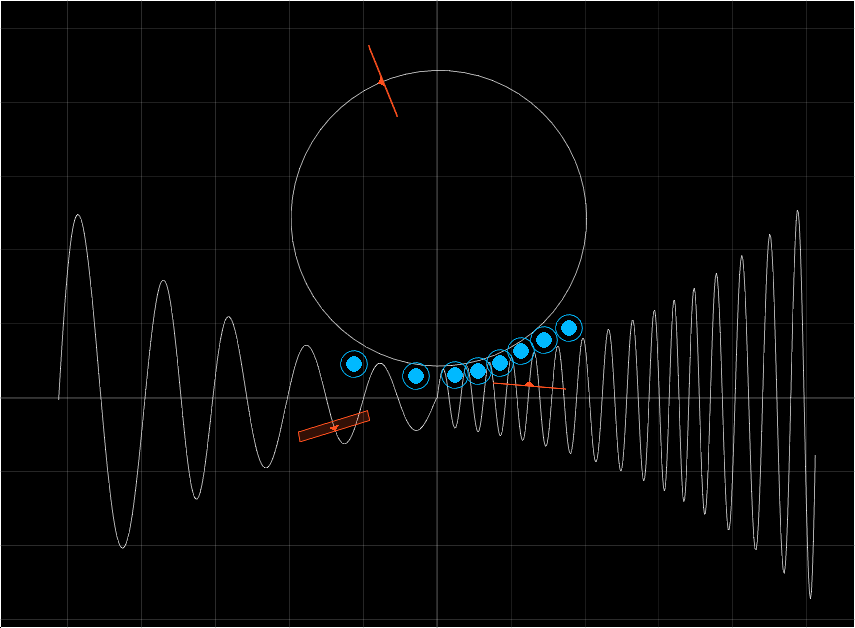
\includegraphics[scale=0.3]{images/iannix.png}
\caption{Une partition composée de trajectoires et de triggers dans le séquenceur graphique IanniX}
\label{fig.iannix}
\end{figure}

\subsubsection{Positionnement d'objets sonores}
Dans un cadre muséographique, on a plus souvent des objets sonores qui peuvent être associés à des éléments graphiques : des notes dans un manuscrit, un personnage sur un tableau... On désire alors contrôler le comportement de cet objet sonore au fil du temps et le scénariser, le faire se déplacer, changer ses propriétés sonores, etc.

Cette approche est aussi plus pertinente dans un cadre vidéo-ludique : en effet, les outils de conception de jeu-vidéo (\textit{citer partie rapport cnam}) ont une approche fortement orientée objet - la méthode actuellement la plus répandue dans l'industrie est le pattern Entity-Component-Systems\footnote{Component Based Engine Design, Randy Gaul : http://www.randygaul.net/2013/05/20/component-based-engine-design/}, qui permet d'encapsuler différentes couches applicatives (qui peuvent contenir des données, des comportements...) très simplement dans n'importe quel objet du jeu.

Voici plusieurs examples d'applications :
\paragraph{Application 1 : Sonopluie}
Ici, des utilisateurs font un parcours dans une ville. Ils ont un casque et sont géolocalisés. En fonction de leur position et de leur parcours, ils entendent des messages rappelant des évènements historiques de la ville. 

De plus, si des utilisateurs se croisent, l'application peut en avoir conscience et déclencher des évènements spécifiques.

Cette application a plusieurs pré-requis : 
\begin{itemize}
\item L'outil de conception doit, au minimum, permettre de placer des points sur une carte et de définir une action sur le périphérique de l'utilisateur, lorsqu'il rencontre un point.
\item Pour plus de richesse, des zones sonores peuvent être définies : par exemple, une bande de plage.
\item Il doit y avoir une notion de scénarisation telle qu'offerte par i-score, permet de construire une histoire au cours du temps, plutôt que de simplement avoir une liste de hot-spots interactifs.
\item Enfin, se pose la question de la répartition et de l'interaction entre plusieurs protagonistes. Une possibilité serait de définir des zones d'interactions qui ne s'activent que lorsque plusieurs participants sont présents à l'intérieur. Les périphériques des utilisateurs présents dans cette zone doivent communiquer entre eux (ou bien communiquer via un serveur, mais cela nécessite des appareils possédant une connection internet).
\end{itemize}

\paragraph{Application 2 : Le promeneur écoutant}

cf. rapport CNAM 

\subsection{Interactivité et interfaces}
Ici, nous nous intéressons aux possibilités de création et de contrôle dynamique d'interfaces graphiques. La plupart des paradigmes d'UI permettent de définir des vues dans un éditeur graphique, mais ces vues sont en général statiques et il est nécessaire de recourir à des langages de programmation pour avoir une évolution dans le logiciel \textit{(à vrai dire il y a des outils graphiques pour ça dans Qt par exemple, j'imagine que ça doit pouvoir se faire assez bien dans Flash aussi ?)}. 

Nous aborderons ici deux cas : le premier est celui des interfaces utilisateur programmables graphiquement, ce qui peut s'avérer utile quand il y a de nombreuses animations et objets graphiques non-usuels. Le second est celui des interfaces nécessaires pour contrôler des espaces de paramètres particuliers.

Il reste des problèmes non abordés : notamment la création d'objets dynamique, la visualisation, et la gestion de comportements d'objets en masse, comme par exemple pour un générateur de particules.

\subsubsection{Contrôle d'interfaces utilisateurs}
Le premier cas est celui d'une application en mode kiosque, possédant un menu de choix des langues, qui mène pour chaque langue à un menu principal permettant de choisir des vidéos à lire en mosaïque.

Lorsqu'une langue est choisie, l'écran principal glisse depuis la droite. Les boutons ont une animation lorsqu'ils sont pressés. Lorsqu'une vidéo est pressée, elle se met en lecture. Des \textit{gestures} permettent de déplacer les vidéos, en suivant des lois de physique basiques (notamment, les vidéos peuvent tourner et rentrer en collision).

(\textit{note:  s'il y a une vraie application muséo à la place ici je suis preneur :) j'ai juste imaginé des choses pour faire un example.})

Les problématiques, ici, sont : 
\begin{itemize}
\item Le contrôle d'un grand nombre d'élements statiques, et la hiérarchisation de ces éléments. Par exemple, si les boutons de langues sont enfants du premier menu, on veut qu'ils suivent le déplacement de leur menu parent.
\item Un questionnement sur les modèles physiques. Cela a déjà été abordé pour les modèles masse-ressort évoqués en spatialisation de musique.
\item La gestion d'animations. Généralement, une animation consiste en l'interpolation de paramètres dans le temps, en passant par des états prédéfinis (keyframes).
\end{itemize}

\subsubsection{Navigation dans espaces de paramètres}

\begin{figure}[h]
\centering
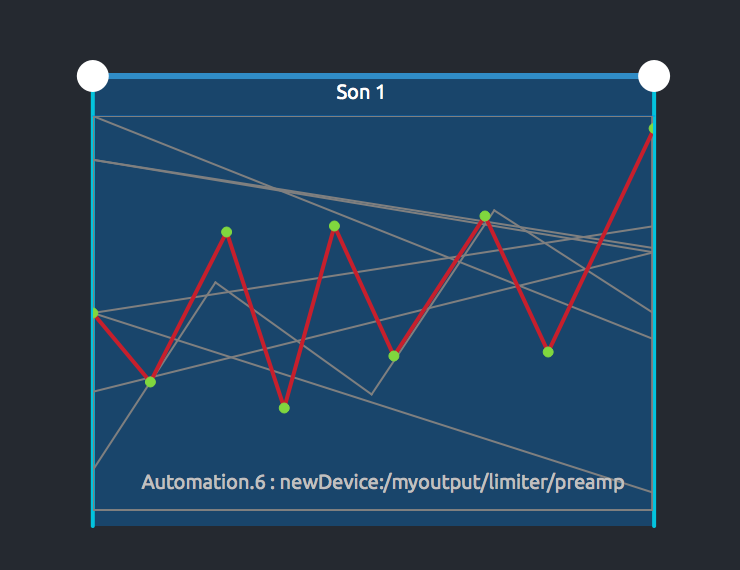
\includegraphics[scale=0.5]{images/iscore.png}
\caption{De nombreux paramètres sur un seul axe dans i-score, rendant la partition peu lisible.}
\label{fig.iscore}
\end{figure}

Un problème plus général est celui de la gestion des espaces de paramètres particuliers.

Par exemple, pour choisir et animer la couleur d'un élément dans le temps, il est nécessaire d'avoir des outils de création adaptés, tout en gardant les primitves de trajectoires et d'objets évoquées précédemment.

Un second point est celui de la gestion des correspondances entre espaces de données. Ainsi, si on désire automatiser un point sur un plan en deux dimensions dans le temps, il doit être possible de le faire selon les systèmes de coordonnées cartésiennes ou polaires.

De même, pour les couleurs il est important de pouvoir travailler en RVB, mais aussi en L*a*b*, HSL, et notamment de pouvoir passer facilement d'un mode à l'autre.

Enfin, le dernier point est le cas d'une aide à l'écriture pour une application comportant un grand nombre de paramètres, potentiellement artistiques. Le problème de la visualisation se pose lorsque ces paramètres sont représentés sur une seule dimension, comme en fig.~\ref{fig.iscore}.

\subsection{L'espace pour le spectacle}
\subsubsection{Danse interactive}
Dans cette application, nous désirons travailler avec plusieurs danseurs sur scène, et produire un comportement émergent au gré de leurs déplacements et du scénario du spectacle.

Le premier cas est très simple : il existe un cercle virtuel et invisible au sol, délimité par l'auteur du spectacle, et on désire allumer une lumière lorsqu'un danseur rentre dans le cercle. C'est similaire au cas de Sonopluie vu plus tôt et se rapporte à un simple test booléen.

Nous aimerions maintenant créer de la géométrie. Soient deux danseurs : la seconde partie du spectacle consiste à allumer la lumière lorsque le barycentre des deux danseurs est dans le cercle virtuel. Cela requiert, en plus  de ce qui a été dit précédemment, de la nécessité d'avoir une géométrie dynamique et définie par des paramètres provenant de l'extérieur.

Enfin, dans la dernière partie du spectacle, nous utilisons la distance entre les deuxs danseurs pour faire varier le rayon du cercle au centre de la scène.

Dans cet exemple, nous avons donc comme caractéristique principale une grande liberté de contrôle laissée à l'auteur, ainsi que la capacité de définir des géométries complexes.

\subsubsection{Contrôle de robots}
Une application intéressante est celle des chorégraphies de robot. Ce chantier, commencé en 2015, vise à étendre les possibilités du séquenceur i-score d'abord à des robots quadrupèdes Metabots (fig.~\ref{fig.metabots}), puis, potentiellement à des drones.

\begin{figure}[h]
\centering
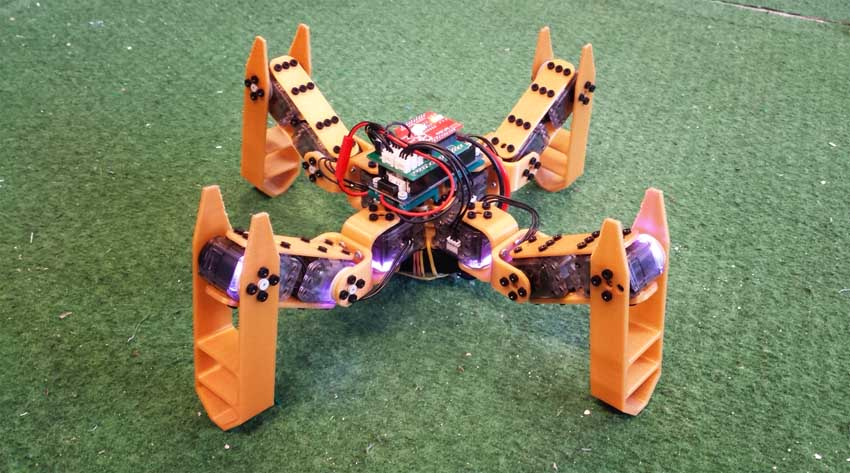
\includegraphics[scale=0.2]{images/spidey.jpg}
\caption{Un metabot.}
\label{fig.metabots}
\end{figure} %TODO mettre sc iscore

Là encore, la question de l'écriture se pose, et notamment le cas de la gestion d'un grand nombre d'objets dans un espace relativement restreint.

De plus, ces objets ne vont pas forcément réagir comme prévu : si par exemple un robot est programmé pour aller tout droit, mais qu'il rencontre un autre robot qui serait tombé en panne sur le chemin, actuellement le premier robot ne saurait en tenir compte et rentrerait en collision avec le second robot.


\section{Réalisations}
Les réalisations se séparent en deux catégories : la première consiste en des extensions pour i-score ou d'autres logiciels et frameworks. Ces logiciels ont été retenus car ils sont directement en lien avec les problématiques qui ont été évoquées précédemment.

Puis, une fois ces cas étudiés, nous avons tenté d'apporter une solution originale au problème d'écriture qui se pose.

\subsection{Clients manipulant des données spatiales}
\subsubsection{Interopérabilité avec Qt}
Un plug-in pour i-score permettant d'exposer l'arbre d'objets d'une application Qt a été développé. Cela permet de contrôler facilement la position et le contenu des éléments d'une interface graphique réalisée avec cette technologie depuis i-score.

\subsubsection{Contrôle d'OpenAL}
OpenAL est une bilbiothèque ayant été développée pour les besoins des jeux vidéos au début des années 2000. Elle se base sur une notion de sources sonores associées à des fichiers sons, qui sont positionnées en trois dimensions, ainsi que d'un listener qui se déplace et perçoit donc les sons plus ou moins forts. Une implémentation récente, \textbf{OpenAL-soft}\footnote{http://kcat.strangesoft.net/openal.html}, permet d'utiliser des HRTF pour avoir une sensation de spatialisation réaliste au casque.  

Un outil exposant des sources OpenAL via le protocole Minuit et permettant de charger des sons, puis de les positionner dans l'espace a été implémenté. Ces sources sont donc contrôlables depuis i-score.

\subsubsection{Contrôle de metabots}
Une couche de communication entre i-score et les robots Metabots
a été développée et a mené à une présentation aux Robot Makers Day, avec notamment 
une chorégraphie ou deux robots sont contrôlés et synchronisés musicalement avec i-score. 

Cela a été l'occasion de comparer le développement d'une chorégraphie entre i-score, et 
un langage de programmation graphique inspiré de Scratch. Les résultats ont été probants : il a fallu 
beaucoup moins de temps pour produire une même chorégraphie dans i-score que dans l'autre langage.


\subsection{État de l'art sur méthodes spatiales, positionnement, trajectoires}

\subsubsection{Free-hand drawing sur tableau}
À titre d'exemple pour des démonstrations et exposés, un outil permettant de dessiner des zones de manières arbitraire sur un tableau a été développé (cf. fig.~\ref{fig.tableau}).

\begin{figure}[h]
\centering
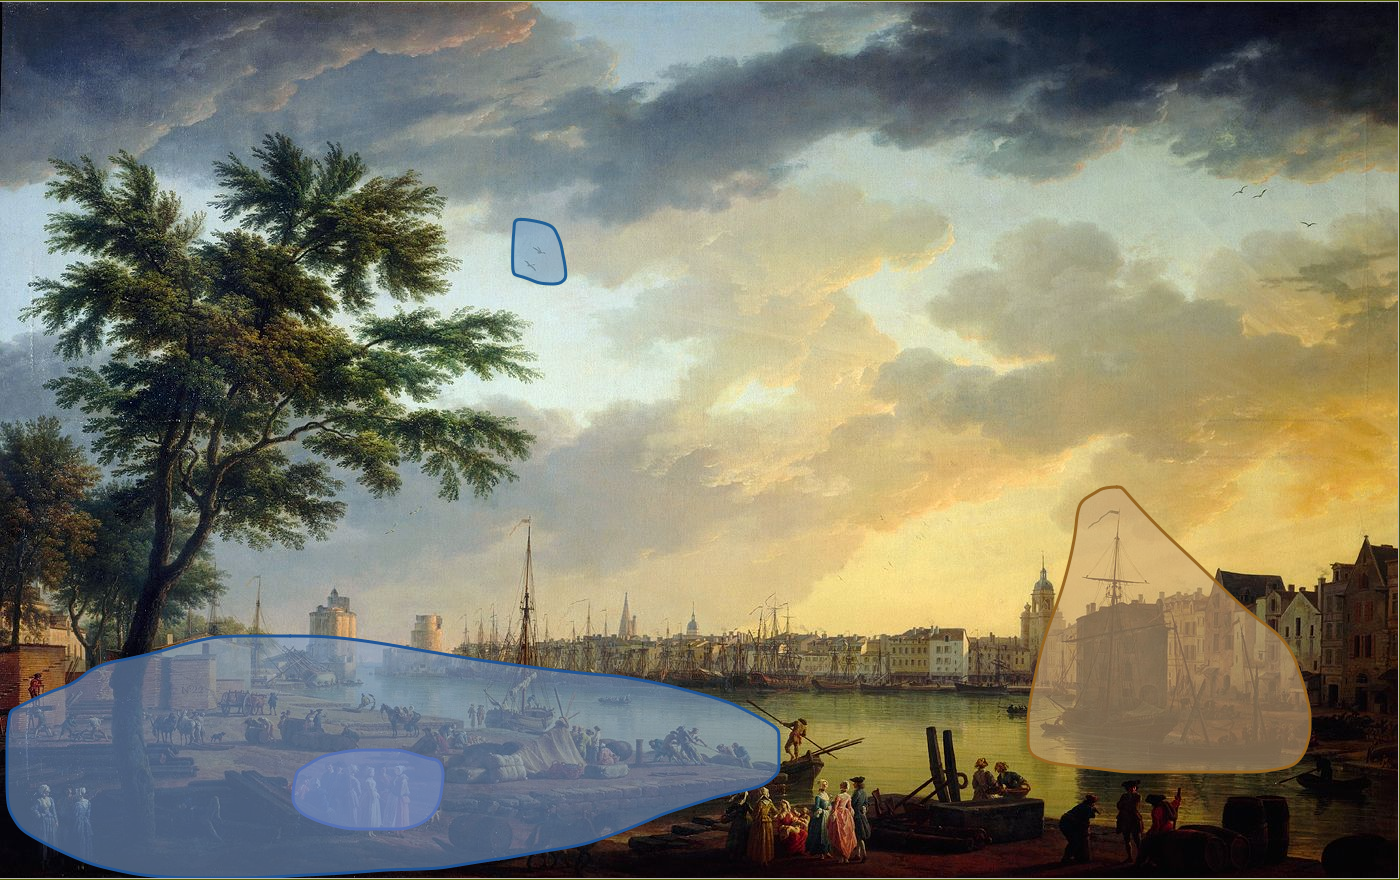
\includegraphics[scale=0.2]{images/harbour.png}
\caption{Un tableau sur lequel on peut apposer des couches sonores.}
\label{fig.tableau}
\end{figure} 

Lorsqu'une zone est activée, elle produit un son qui peut être en relation avec les éléments sous-jacents. % TODO mettre minuit là dedans ?

\subsubsection{Liste des tâches et prototype pour processus de mapping spatial}
Suite aux différents cas d'utilisation qui ont été présentés, un état de l'art % TODO citer num. annexe
a été effectué dans le domaine de l'authoring spatial, et des techniques et méthodes possibles.

Cet état de l'art a ensuite conduit à la recherche de méthodes possibles pour combler le besoin existant pour un outil permettant de spécifier des scénarios manipulant beaucoup de données spatiales entrelacées entre elles, ainsi qu'avec une évolution temporelle.

Le premier point auquel nous nous intéressons est celui du modèle de données. Il existe deux courants : les approches orientées langage, et les approches orientées données. 

Les premières sont des langages de programmation spécifiquement étudiés pour résoudre le problème posé de manière élégante. Plusieurs possibilités ont été étudiées : 
\begin{itemize}
\item Utiliser un langage de script existant, tel que Lua, Python ou JavaScript pour définir les objets et comportements spatiaux. L'avantage est une très grande flexibilité, mais les capacités d'analyse statique et d'optimisation sont diminuées si l'intégralité du langage est accessible à l'utilisateur.
\item Il existe une famille de langages plus spécialisés dans la gestion de données interactives : c'est le courant de la programmation fonctionnelle réactive\footnote{\textit{Arrows, robots, and functional reactive programming}, 2003, Paul Hudak}.
\item Un DSL (langage spécifique à un domaine) pensé pour la création de graphismes vectoriels est présent dans le package Haskell \textsc{diagrams}. Il fonctionne à l'aide d'un jeu de primitives réduites qui doivent être composées par la suite.
\item L'approche que nous avons pour l'instant retenue est d'utiliser un système de calcul symbolique\footnote{En pratique le choix s'est porté sur GiNaC : \url{www.ginac.de}}. Ainsi, le langage utilisé est simple : ce sont les mathématiques traditionnelles. L'avantage est la relative simplicité à l'utilisation par rapport à la nécessité d'apprendre un langage complet, ainsi que la possibilité de changer de moteur de résolution si celui choisi n'offre pas les performances adéquates.
En revanche, il n'est plus possible de gérer des cas comme des boucles, etc.
\end{itemize}

En parallèle, les approches orientées données sont souvent plus adaptées à une manipulation directe par un utilisateur novice, car elles sont basées sur des outils graphiques, ou de plus haut niveau : 
\begin{itemize}
\item Il existe des modèles qualitatifs de représentation des données spatiales : RCC-8, OPRA-4, etc. Ces modèles sont principalement étudiés dans le monde de l'intelligence artificielle et de l'ingénierie des connaissances. Ils sont notamment utilisés pour de la reconaissance d'images, de lieus, etc.
\item Le parc de logiciels graphiques existant se base souvent sur quelques primitives simples qui sont ensuites composées entre elles, ainsi que sur l'utilisation de modèles 3D, comme pour Maya en figure~\ref{fig.maya}.

\end{itemize}

\begin{figure}[h]
\centering
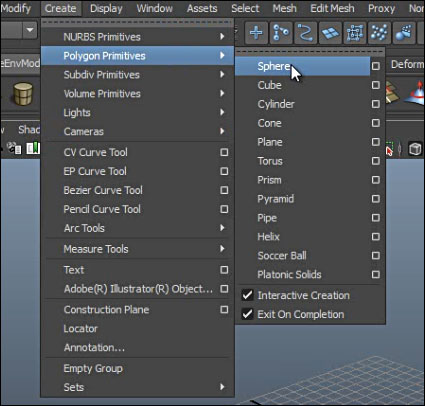
\includegraphics[scale=0.5]{images/maya.jpg}
\caption{Primitives graphiques dans le logiciel de 3D Maya.}
\label{fig.maya}
\end{figure} 

La méthode que nous proposons combine les deux : utiliser un CAS pour spécifier des objets de base avec les quels travailler, puis permettre à l'utilisateur de faire des transformations graphiques - translation, rotation, scale - sur les objets. Les paramètres de ces objets sont extraits de la formule mathématique et séparés en deux ensembles : ceux qui font partie de l'espace d'évaluation et ceux qui font partie de l'espace de paramétrisation. Par la suite, des propriétés peuvent être extraites à l'aide d'algorithmes intervenant plus tard, comme la collision entre deux objets. Ces propriétés sont ensuites utilisables dans le reste d'i-score via l'arbre de paramètres.

Le rendu se fait actuellement par un algorithme naïf de pixelisation, qui devra par la suite être étendu à de la voxelisation pour une manipulation en trois dimensions. Pour des objets définis dans plus de de trois dimensions, il est possible de choisir la restriction que l'on visualise. 

La manipulation et l'édition des objets ainsi créé est faite via l'édition de l'équation de manière textuelle, et nous désirons étudier les interactions utilisateur possibles pour une édition via des modalités purement graphique. 


\section{Conclusion}

Problèmes restants : question de visualisation / rendu, etc.

\printbibliography
\end{document}